	% Welcome! This is the unofficial University of Udine beamer template.

% We defined four theme colors: UniBrown, UniBlue, UniGold
% and UniOrange. For example, to write some uniud-brownish
% text, just use: \textcolor{UniBrown}{Hello!}

\documentclass[usenames,dvipsnames, 10pt]{beamer}

\usepackage{tikz}
\usetikzlibrary{arrows.meta}

\usepackage[utf8]{inputenc}
\usepackage{algorithm2e}
\usepackage{verbatim}
\usetheme{uniud}
%\bibliography{bib}
%%% Bibliography
%\usepackage[style=authoryear,backend=biber]{biblatex}
%\addbibresource{bib.bib}
\usepackage{tikz}
\usetikzlibrary{patterns,snakes}
%\DeclareNameAlias{author}{first-last}
\newcommand{\dataset}{{\cal D}}
\newcommand{\fracpartial}[2]{\frac{\partial #1}{\partial  #2}}
\makeatletter
\newcommand{\distas}[1]{\mathbin{\overset{#1}{\kern\z@\sim}}}%
\newsavebox{\mybox}\newsavebox{\mysim}
\newcommand{\distras}[1]{%
	\savebox{\mybox}{\hbox{\kern3pt$\scriptstyle#1$\kern3pt}}%
	\savebox{\mysim}{\hbox{$\sim$}}%
	\mathbin{\overset{#1}{\kern\z@\resizebox{\wd\mybox}{\ht\mysim}{$\sim$}}}%
}
\makeatother
%%% Suppress biblatex annoying warning
\usepackage{silence}
\WarningFilter{biblatex}{Patching footnotes failed}

%%% Some useful commands
% pdf-friendly newline in links
\newcommand{\pdfnewline}{\texorpdfstring{\newline}{ }} 
% Fill the vertical space in a slide (to put text at the bottom)
\newcommand{\framefill}{\vskip0pt plus 1filll}
\newcommand{\bigCI}{\mathrel{\text{\scalebox{1.07}{$\perp\mkern-10mu\perp$}}}}
\newcommand\asto{\mathrel{\stackrel{\makebox[0pt]{\mbox{\normalfont\tiny a.s.}}}{\to}}}


\newcommand{\independent}{\mbox{${}\perp\mkern-11mu\perp{}$}}
\newcommand{\notindependent}{\mbox{${}\not\!\perp\mkern-11mu\perp{}$}}
\newcommand{\iid}{\overset{\text{iid}}{\sim}}

\newcommand{\R}{\mathbb{R}}
\newcommand{\E}{\mathbb{E}}
%\newcommand{\C}{\mathbb{C}}

\newcommand{\y}{\mathbf{y}}
\newcommand{\uu}{\mathbf{u}}
\newcommand{\z}{\mathbf{z}}
\newcommand{\vv}{\mathbf{v}}
\newcommand{\w}{\mathbf{w}}
\newcommand{\x}{\mathbf{x}}

\newcommand{\Hyp}{\mathcal{H}}
\newcommand{\Myp}{\mathcal{M}}
\newcommand{\Ayp}{\mathcal{A}}

\newcommand{\Yspace}{\mathcal{Y}}
\newcommand{\Xspace}{\mathcal{X}}


\newcommand{\RR}{\mathbb{R}}

\title[Information-Theoretic Analysis of Learning Algorithms]{‌\vspace{0.5cm}\\
Information-Theoretic Analysis of Learning Algorithms}
\author[Behrad ]{
  Behrad Moniri
  \pdfnewline
  \texttt{bemoniri@ee.sharif.edu}
}
\institute{\small{EE Department - Sharif University of Technology}}
\date{February 8, 2021}
\begin{document}

\begin{frame}
\titlepage
\end{frame}

\begin{frame}
	\frametitle{Overview of Talk}
	
	\textbf{Goal}: Analysis of the performance of learning algorithms using tools from information theory.
	\pause
	
	\vspace{1cm}
	\begin{enumerate}
		\item Frequentist Setting.
		\item Bayesian Setting.
	\end{enumerate}
\end{frame}

\section{Frequentist Setting}
\framecard{\LARGE Frequentist Setting}



\begin{frame}
	\frametitle{Problem Formulation}
	
	\begin{itemize}
		\item 
		
		
		\textbf{Instance Set}: $\mathcal{Z}$ \\ \textbf{Hypothesis Set}: $\mathcal{W}$ \\
		\textbf{Loss Function}:
		$\ell: \mathcal{W}\times \mathcal{Z} \to \R^+$
		
		\pause
		\item An unknown distribution  $\mu$ on $\mathcal{Z}$.			
		
		\pause
		\item Given $S = (Z_1, \dots, Z_n)\sim \mu$.
		
		
		\pause
		\item For every $w \in \mathcal{W}$, define
		\begin{equation*}
		\begin{cases}
			L_\mu(w) = \E_\mu[\ell(w, Z)] = \int \ell(w, z) \mu(dz)\\
			\\
			L_S(w) = \frac{1}{n}\sum_{i = 1}^{n} \ell(w, Z_i)
		\end{cases}
		\end{equation*}
	
		\pause
		\item \textbf{Goal}:  Algorithm picks $W \in \mathcal{W}$ according to some $P_{W|S}$. Control
			\begin{equation*}
				\E [\mathrm{gen}(W)] =  \E [L_\mu(W) - L_S(W)],
			\end{equation*}
			where the expectation is over $P_{S, W} = \mu^{\otimes n}  P_{W|S}$.		
	\end{itemize}
	
\end{frame}


\begin{frame}
	\frametitle{History}
	
	\begin{itemize}
		\item Traditional ways of analyzing generalization:
		\begin{itemize}
			\item VC Dimension
			\item Radamacher Complexities
		\end{itemize}
		
		\pause
		
		\item \textbf{Uniform Bounds}: $\E[\mathrm{gen}(W)] \leq \E[\sup_{w\in\mathcal{W}} \mathrm{gen}(w)]$
	
	
		\pause
		
		\item These bounds depend only on the hypothesis set: \textbf{pessimistic}.
		
		\pause
				
		\item \textbf{Intuition}:
		\begin{center}
			less information usage from $S$ $\implies$ less overfitting
		\end{center}
		 	
	\end{itemize}
\end{frame}

\begin{frame}
	\frametitle{Decoupling Estimate}
		\begin{block}{Definition}
		The random variable $X$ is called $\sigma$-subgaussian if
		\begin{small}
			\begin{equation*}
			\forall \lambda \in \R: \;\; \E\Big[e^{\lambda(X - \E[X])}\Big] \leq e^{\lambda^2\sigma^2/2}.
			\end{equation*}
		\end{small}
		\vspace{-0.5cm}
	\end{block}
	\pause
	\begin{alertblock}{Lemma {\scriptsize[Xu and Raginsky,  2017] \& [Russo and Zou,  2016]}}
		Let $(X, Y) \sim P_{XY}$, and $\bar{Y} \sim P_Y$ be independent copy. For any real valued $f:\mathcal{X}\times \mathcal{Y} \to \R$, if $f(X, \bar{Y})$ is $\sigma$-subgaussian, then
		\vspace{-0.3cm}		
		\begin{equation*}
			\big|\E[\,f(X, Y)] - \E[\,f(X, \bar{Y})]\big| \leq \sqrt{2\sigma^2I(X;Y)}
		\end{equation*}
		\vspace{-0.5cm}
	\end{alertblock}
	\vspace{-0.4cm}
	\begin{columns}
		\begin{column}{0.5\textwidth}
		\end{column}
		\begin{column}{0.5\textwidth}  %%<--- here
			\begin{center}
			\begin{small}
				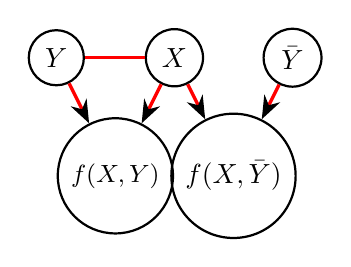
\begin{tikzpicture}
				\begin{scope}[every node/.style={circle,thick,draw}]
				\node (X) at (1.5,0) {$X$};
				\node (Y) at (0,0) {$Y$};
				\node (Ybar) at (3,0) {$\bar{Y}$};
				\node (f) at (0.75,-1.5) {\small $f(X, Y)$};
				\node (fbar) at (2.25,-1.5) {$f(X, \bar{Y})$};
				\end{scope}		
				\begin{scope}[>={Stealth[black]},
				every node/.style={fill=white,circle},
				every edge/.style={draw=red,very thick}]
				\path [->] (X) edge (fbar);
				\path [-]  (X) edge (Y);
				\path [->] (X) edge (f);
				\path [->] (Y) edge (f);
				\path [->] (Ybar) edge (fbar);
				\end{scope}
				\end{tikzpicture}			
			\end{small}
		\end{center}
		\end{column}
	\end{columns}
\end{frame}

\begin{frame}
	\frametitle{Decoupling Estimate}
	\textbf{Proof}: Donsker-Varadhan variational representation: 
	\vspace{-0.2cm}		
	\begin{equation*}
	\mathrm{KL}(\pi||\rho) = \sup_F \Big\{\int_\Omega F d\pi - \log\int_\Omega e^F d\rho\Big\}.
	\end{equation*} 
	\pause
	\vspace{-0.2cm}		
	For any $\lambda \in \R$, we have
	\begin{align*}
	\mathrm{KL}(P_{XY}||P_X\otimes P_Y) &\geq \E[\lambda f(X, Y)] - \log \E[e^{\lambda f( X, \bar Y)}]\\
	&\geq \lambda\E[\,f(X, Y)] - \lambda\E[\,f( X, \bar Y)] - \frac{\lambda^2\sigma^2}{2}
	\end{align*}	
	\pause
	Discriminant must be non-positive, which concludes the proof.\qed
\end{frame}

\begin{frame}
	\frametitle{Capacity Theorem}
	
	\begin{itemize}
		\item Let $f(s, w) = \frac{1}{n} \sum_{i = 1}^{n} \ell(w, z_i)$. \pause  We have
		\vspace{-0.1cm}
		\begin{align*}
		\E [\mathrm{gen}(W)] &= \E[L_\mu(W) - L_S(W)]\\ 
		&= \E[\,f(\bar S,  W)] - \E[\,f( S,  W)].
		\end{align*}
		\pause
		\vspace{-0.5cm}
		\item If $l(w, Z)$ is $\sigma$-subgaussian $\implies$ $f(S, w)$ is $\frac{\sigma}{\sqrt{n}}$-subgaussian.
	\end{itemize}
	
	\vspace{-0.1cm}
	\pause
	\begin{block}{Theorem {\scriptsize [Xu and Raginsky,  2017]}}
		Suppose that $\ell(w, Z)$ is $\sigma$-subgaussian for $\mu$, under all $w\in\mathcal{W}$. We have
		\vspace{-0.2cm}
		\begin{equation*}
			|\E [\mathrm{gen}(W)]| \leq \sqrt{\frac{2\sigma^2}{n} I(S;W)}
		\end{equation*}
		\vspace{-0.4cm}
	\end{block}
	\pause	
	\begin{alertblock}{Remark}
		\begin{itemize}
			\item The learning algorithm
			$P_{W|S}$: \textbf{channel} from $S$ to ${W}$.
			
			\item $\sup_{\mu} I(S; W)$:		
			channel \textbf{capacity} of the channel, under the constraint that the input distribution is of a product form.
			
		\end{itemize}			
	\end{alertblock}	
\end{frame}


%\begin{frame}
%	\frametitle{Some Applications: Gibbs Algorithm}
%		\begin{itemize}
%			\item \textbf{Idea}: Minimizes the empirical risk regularized by $I(S;W)$.
%			$$P_{W|S}^\star = \arg\min_{P_{W|S}} \Big(\E[L_S(W)] + \frac{1}{\beta} I(S;W)\Big) \implies \text{  depends on } \mu.$$
%			\pause
%			\item  Use $I(S;W) \leq D(P_{W|S}||Q | P_S) = I(S;W) + D(P_W||Q)$. 
%			\begin{align*}
%				&\min_{P_{W|S}} \Big(\E[L_S(W)] + \frac{1}{\beta} D(P_{W|S}||Q | P_S)\Big)\\
%				&= 	\min_{P_{W|S}}	\int_{\mathcal{Z}^n} \mu^{\otimes n}(ds) \Big(\E[L_s(W)|S=s] + \frac{1}{\beta}D(P_{W|S=s}||Q)\Big)
%			\end{align*}
%			\pause
%			\item Hence
%			\begin{equation*}
%				P_{W|S}^\star = \arg\min_{P_{W|S}} \Big(\E[L_s(W)|S=s] + \frac{1}{\beta}D(P_{W|S=s}||Q)\Big).
%			\end{equation*}			
%		\end{itemize}
%\end{frame}
%
%\begin{frame}
%	\frametitle{Some Applications: Gibbs Algorithm}
%	\begin{alertblock}{Gibbs Algorithm}
%		Suppose $\mathcal{W}$ is countable. Let $w_0$ denote the hypothesis that achieves the minimum population risk among $\mathcal{W}$. For $l \in [0, 1]$, the population risk of $\mathcal{W}$ satisfies:
%		
%		\begin{equation*}
%			\E[L_\mu(W)] \leq \inf_{w\in\mathcal{W}}L_\mu(w) + \frac{1}{\beta}\log\frac{1}{Q(w_0)} + \frac{\beta}{2n}.
%		\end{equation*}
%	\end{alertblock}
%
%	\pause
%	
%	\textbf{Other idea}: Noisy ERM, $\dots$.
%\end{frame}



\begin{frame}
	\frametitle{Chaining Mutual Information}
	\begin{itemize}
		\item When $W$ is deterministic given $S$: $I(S; W)$ is infinite.
		\pause
		\item \textbf{Can we tighten our bounds?}
		\pause
		
		\item Assume we intend to upper bound $\E\Big[\sup_{t \in T} X_t\Big]$.
		
		\item $(T, d)$ is a metric space. $X_t - X_s \sim d^2(s, t)$-subgaussian.
		\pause
		\begin{columns}
			\begin{column}{0.5\textwidth} 
				\hspace{1cm} Let $\mathcal{N}_k$ be $\epsilon_k = 2^{-k}$-net of $T$ 
				
				%\hspace{1cm} $\pi_k(t) = \arg\min_{x \in \mathcal{N}_k} d(x, t)$	
			\end{column}
			\begin{column}{0.5\textwidth} 
%				\begin{figure}
%					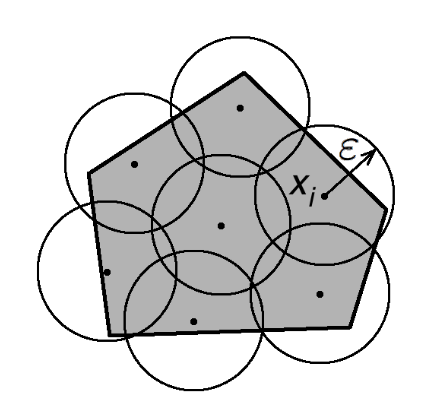
\includegraphics[scale=0.2]{cover.png}
%				\end{figure}
			\end{column}
		\end{columns}
		
		%	\item 
		%	$$X_t = X_{\pi_1(t)} + \big(X_{\pi_2(t)} - X_{\pi_1(t)}\big) + \dots + \big(X_{\pi_d(t)}-X_{\pi_{d-1}(t)}\big) + \big(X_t - X_{\pi_d(t)}\big).$$ 	
		
		\pause
		\textbf{Dudley bound}: multi-scale approximation of $T$
		\begin{equation*}
		\E\Big[\sup_{t \in T} X_t\Big] \leq 6 \sum_{k \in \mathbb{Z}} 2^{-k} 	\sqrt{\log \mathcal{N}(T, d, 2^{-k})}.
		\end{equation*}
		
	\end{itemize}	
\end{frame}


\begin{frame}
	\frametitle{Chaining Mutual Information}
			\begin{exampleblock}{Chaining Mutual Information {\scriptsize[Asadi, Abbe \& Verdu. 2019]}}
			 If $\{\mathrm{gen}(w)\}_{w\in\mathcal{W}}$ is a subgaussian process in $(\mathcal{W}, d)$:
			\begin{equation*}
			\E[\mathrm{gen}(W)] \leq 3\sqrt{2} \sum_{k = k_1(\mathcal{W})}^{\infty} 2^{-k} \sqrt{I(\pi_k(W); S)}.
			\end{equation*}		
			\vspace{-0.4cm}	 
		\end{exampleblock}
\end{frame}


%\begin{frame}
%	\frametitle{Applications}
%	
%	\begin{itemize}
%		\item \textbf{Take away}: We should control $I(S; W)$ for good generalization.
%		\vspace{1cm}
%		\pause
%		\begin{itemize}
%			\item Noisy ERM. {\scriptsize [Xu \& Raginsky, 2017]}
%			\item Regularize $I(W; S)$ or proxies of it. {\scriptsize [Assadi \& Abbe, 2020]}
%		\end{itemize}
%	\end{itemize}
%\end{frame}
\section{‌Bayesian Setting}
\framecard{\LARGE ‌Bayesian Setting}

\begin{frame}
	\frametitle{‌Bayesian Learning}
	
	
	
	\vspace{0.4cm}
	
	\begin{itemize}
		\item \textbf{Generation Model}: 
			\begin{align*}
			&P_{W, S, Z} = P_W \otimes \prod_{i = 1}^{n} P_{Z_i|W} \otimes P_{Z|W}\\ &\forall\, i \in [n], \;\; P_{Z_i|W} = P_{Z|W}			
			\end{align*}
		
		
		\vspace{0.3cm}
		
		\item \textit{Predicting Modeling Framework}: $Z = (X, Y)$, and $Z_i = (X_i, Y_i)$.				
		$$P_{Z|W} = P_X \otimes P_{Y|X, W}$$
		
		
		
		\vspace{0.4cm}
		\pause
		\item \textbf{Goal}: predict $Y$ based on $X$ and observations $S = \{Z_1, \dots, Z_n\}$. 

	\end{itemize}
\end{frame}

\begin{frame}
	\frametitle{Minimum Excess Risk}
	\begin{itemize}
		\item \textbf{Generalized Entropy}: 
		
		$$R_{\ell}(Y|X)= \inf_{\psi:\mathcal{X}\to\mathcal{Y}} \E[\ell(Y,\psi(X)] \pause \leadsto  \psi^*_{Y|X}(x).$$
		\pause
		
				\item \textbf{Minimum Excess Risk (MER)}:
		\begin{equation*}
		\mathrm{MER}_\ell^n = R_\ell(Y|S, X) - R_\ell(Y|W, X)
		\end{equation*}
		\pause
		\vspace{-0.5cm}
		\item MER is algorithm \textit{independent}.
		\pause
		\begin{exampleblock}{Theorem {\scriptsize[Xu \& Raginsky 2020],  [Hafez \& Moniri, 2021]}} The following bound can be derived for MER:
			\begin{align*}
			\text{MER}_\ell^n \le \sqrt{\frac{b^2}{2} I(Y;W|S,X) }.
			\end{align*}
		\end{exampleblock}
		
%		\item \textbf{Data Processing}: Assume that $Y - W - V $ holds. We have			
%			\begin{equation*}
%				R_\ell(Y|V) \geq R_\ell(Y|W)
%			\end{equation*}
%		\pause
%		\vspace{-0.5cm}
%		\item Looseness of the inequality:
%		\begin{alertblock}{Lemma {\scriptsize[Xu \& Raginsky 2020]}}
%			Let $\ell:\mathcal{Y}\times \mathcal{Y} \to [0,b]$ be a non-negative bounded function:
%			\vspace{-0.3cm}
%			\begin{equation*}
%			R_\ell(Y|V) - R_\ell(Y|W) \le \sqrt{\frac{b^2}{2}I(Y;W|V)}.
%			\end{equation*}
%			\vspace{-0.3cm}
%		\end{alertblock}	
				%\pause
		%\item \textbf{Minimum Excess Risk}:
		%\begin{equation*}
		%	\text{MER}_\ell ^n = R_\ell(Y|Z^n,X) - R_\ell(Y|W).
		%\end{equation*}		
	\end{itemize}	
\end{frame}

%\begin{frame}
%	\frametitle{Minimum Excess Risk}
%	\begin{itemize}
%
%
%	\end{itemize}	
%\end{frame}

\begin{frame}
	\frametitle{Minimum Excess Risk: Lower Bounds}
	\begin{itemize}
		\item Lower bounds were left as an open problem in {\scriptsize[Xu \& Raginsky 2020]}.
		\pause
		\begin{block}{Remark {\scriptsize[Hafez \& Moniri 2020]}}
			It is \textit{impossible} to find a matching lower bound such that
			\begin{equation*}
				\text{MER}_\ell^n \geq \alpha\sqrt{I(Y; W | S, X)}.
			\end{equation*}
		\end{block}
		%\pause
		%Consider the toy problem:
		%\pause
		%\begin{small}
		%	\begin{equation*}
		%	\begin{cases}
		%	W_1, W_2\distas{\text{i.i.d.}} U(-1,1),\\
		%	\epsilon_1 = 0,\;\; \epsilon_2 \distas{} U(-1,1)\\
		%	Y=(Y_1,Y_2)=(W_1+\epsilon_1, W_2+\epsilon_2).
		%	\end{cases}
		%	\end{equation*}
		%\pause
		%\end{small}
		%\item Define $\ell((y_1,y_2), (\hat{y}_1,\hat{y}_2))= (y_1-\hat{y}_1)^2$.    
		
		
		%\item In this case,  $\forall n>1, \mathrm{MER}_\ell^n = 0$. % MER will be zero 
		%\item $I(W;(Y_1,Y_2)|Z^n)\ge I(W;Y_2|Z^n)$ approaches zero as $n\to \infty$.%, 
		
	\end{itemize}
\end{frame}


\begin{frame}
	\frametitle{Minimum Excess Risk: Lower Bounds}
	\begin{itemize}		

%		\item \textbf{Rate-Distortion theory}: 
%		\begin{align*}
%		D(R)= \inf_{P_{\hat{X}|{X}}} \E[d(X,\hat{X})]
%		\;\; \mathrm{s.t.}\;\; I(X; \hat{X})\le R. 		
%		\end{align*}
								
%		\pause
		
		\item Define the following distortion function:
		\begin{equation*}
		\label{eq:d-def}
		d(w,\hat{h}(.)) = \E_{XY|W=w} [\ell(Y,\hat{h}(X))-\ell(Y,\psi^*_{Y|XW}(w, X))].
		\end{equation*}

		\pause
		
		\item \textbf{Optimal algorithm}: outputs $\hat{h}(.)= \psi^*_{Y|SX} (s, .)$.
		
		\begin{align*}
		\E_{WS}[&d(W,\psi^*_{Y|SX}(S, .))] \\
		&= \E_{WSXY}[\ell(Y,\psi^*_{Y|SX} (S, X)) -\ell(Y,\psi^*_{Y|WX}(W,X))]
		\\ &= R_\ell(Y|S,X) - R_\ell(Y|W,X) = \text{MER}_\ell^n.				
		\end{align*}
		


	\end{itemize}
\end{frame}

\begin{frame}
	\frametitle{Minimum Excess Risk: Lower Bounds}
	\begin{itemize}

	\item Define the (constrained) rate-distortion optimization:
	% \begin{equation}
	% D(R)=  
	% \underset{s.t.\; I(W;\hat{h})\le R}{\inf_{P_{\hat{h}}^{Z^n}}} \EX[d(W,\hat{h})].
	% \end{equation}
	\begin{align}
	\label{eq:rate_distortion_base}
	D_n(R)= \inf_{P_{\hat{h}|S}} \E[d(W,\hat{h})], \;\;
	\mathrm{s.t.}\;\; I(W;\hat{h})\le R. \nonumber
	\end{align}
	
	\pause
	
	\item Note that $W \to S \to \hat{h}$ and $P_{S|W}$ is fixed.
	
	\end{itemize}

\begin{block}{Theorem}
	For a given training set size $n$, for all rates $R\ge I(W;S)$, we have 
	\begin{equation*}
	D_n(R) = \mathrm{{MER}}_\ell^n.
	\end{equation*}
\end{block}
\end{frame}

\begin{frame}
	\frametitle{Explicit Bounds on MER}
	Assume that $\mathcal{W}$ is a $d$-dimensional subset of $\R^d$.
	
	\vspace{0.5cm}
	
	\begin{itemize}
		\item \textbf{Upper Bounds} under some regularity conditions on $P_{Z|W}$:
		\begin{itemize}
			\item $\mathrm{MER}_l^n = O(\frac{1}{n})$ for bounded loss.			
			\vspace{0.2cm}
			
			\item $\mathrm{MER}_2^n = O(\frac{1}{n})$ for quadratic loss.
			
		\end{itemize}		 
		 \pause
		 \item  \textbf{Lower Bounds} using the R/D view and the Shannon Lower Bound, in some cases, we prove $\Omega(\frac{1}{n})$ rates.
		 \pause
		 \item For example, in $Y = W^\top X  + \sigma \nu$ with 
		 
		 \begin{equation*}
		 	\begin{cases}
			 	W \sim \mathcal{N}(0, I_{p\times p})\\
			 	X \sim \mathcal{N}(0, \Sigma_X)\\
			 	\nu \sim \mathcal{N}(0, I_{p\times p})
		 	\end{cases}
		 \end{equation*}		 		 
		  we have $\mathrm{MER}_2^n = \Omega(\frac{p}{n})$.
	\end{itemize}
	
	
\end{frame}


\begin{frame}
	\frametitle{Conclusion}
	Using information theoretic tools:
	
	\vspace{0.5cm}
	\begin{itemize}
		\item We upper bounded generalization gap in a frequentist setting.
		\item We upper and lower bounded minimum excess risk in Bayesian statistics.
	\end{itemize}
\end{frame}

\begin{frame}
	\frametitle{References}
	\begin{scriptsize}
	\begin{enumerate}
		\item Aolin Xu and Maxim Raginsky.\\
		\textit{Minimum Excess Risk in Bayesian Learning}\\
		\textbf{Arxiv}, 2020
		
		\item Aolin Xu and Maxim Raginsky.\\
		\textit{Information-Theoretic Analysis of Generalization Capability of Learning Algorithms}\\
		\textbf{NeurIPS}, 2017\\
		
		\item Daniel Russo and James Zou.\\		
		\textit{How much does you data exploration overfit?}\\
		\textbf{AISTAT} 2016, \textbf{IEEE Trans. Info. Theory} 2020\\
		
		\item  Amir R. Asadi, Emmanuel Abbe, and Sergio Verdu.\\		
		\textit{Chaining Mutual Information and Tightening Generalization Bounds}\\
		\textbf{NeurIPS} 2019
		
		\item Hafez-Kolahi, Golgooni, Kasaei, and Soleymani.\\
		\textit{Conditioning and Processing: Thechniques to improve information theoretic generalization bounds}\\
		\textbf{NeurIPS}, 2020.
		
		\item Bu, Zou, and Veeravalli.\\
		
		\textit{Tightening Mutual Information Based Bounds on Generalization Error}\\		
		\textbf{IEEE Sel. Areas in Info. Theory}, 2020.
		
		
		\item Assadi \& Abbe.\\		
		\textit{Maximum Multiscale Entropy and Neural Network Regularization}\\		
		\textbf{Arxiv}, 2020.
	\end{enumerate}
	\end{scriptsize}
\end{frame}

\end{document}